\begin{enumerate}
\item  See Fig. \ref{fig:1.2.6_triangle_1} generated using the following python code
\begin{lstlisting}
solutions/6/codes/triangle/triangle1.py
\end{lstlisting}
\begin{align}
ar\brak{\triangle ABC} &= \frac{1}{2}\norm{(\vec{B}-\vec{A})\times(\vec{C}-\vec{A})}
\\
&=\frac{1}{2}\norm{\myvec{-3\\-3} \times \myvec{0\\-7}} = \frac{21}{2}
\end{align}
and verified by
\begin{lstlisting}
solutions/6/codes/triangle/tri_area_ABC.py
\end{lstlisting} 
%
\begin{figure}[!ht]
\centering
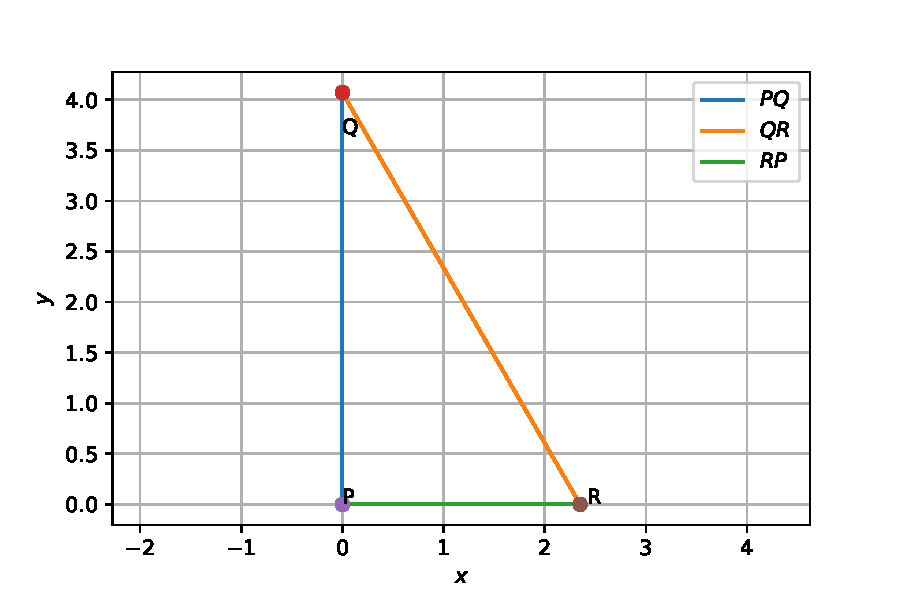
\includegraphics[width=\columnwidth]{./solutions/6/codes/triangle/triangle1.eps}
\caption{Triangle $ABC$ using python}
\label{fig:1.2.6_triangle_1}
\end{figure} 

\item See $\triangle{PQR}$ in Fig. \ref{fig:1.2.6_triangle_2}   generated using the following python code
\begin{lstlisting}
solutions/6/codes/triangle/triangle2.py
\end{lstlisting}
%
\begin{align}
ar\brak{\triangle PQR} &=\frac{1}{2}\norm{(\vec{Q}-\vec{P})\times(\vec{R}-\vec{P})}
\\
&=\frac{1}{2}\norm{\myvec{8\\-4} \times \myvec{10\\3}} = \frac{64}{2}
\end{align}
and verified by 
\begin{lstlisting}
solutions/6/codes/triangle/tri_area_PQR.py
\end{lstlisting} 
%
\begin{figure}[!ht]
\centering
\includegraphics[width=\columnwidth]{./solutions/6/codes/triangle/triangle2.eps}
\caption{Triangle $PQR$ using python}
\label{fig:1.2.6_triangle_2}
\end{figure} 
\end{enumerate}
